%\emph{Machine learning} [is the study of|studies] algorithms that [build|create][mathematical] models of a population or [a] function of interest and estimate their parameters from data  in order to make [good] predictions or inferences.
\emph{Machine learning} is the study of algorithms that build models of a population or function of interest estimating their parameters from data in order to make predictions or inferences. A machine learning expert knows how to choose the right model for the problem in hand (\emph{model selection}), how to efficiently estimate its parameters from the available data (\emph{learning} or \emph{training phase}) and how to evaluate the trained model (\emph{testing phase}).

Machine learning problems divide into three categories depending on the data used to train the model: \emph{supervised learning}, where we learn a function $f(x)$ using examples labelled with their correct output, for instance, learning to estimate the price of a house given its size and number of bedrooms from a data set of houses and their true valuations; \emph{unsupervised learning}, where we look for relationships and structure in unlabelled data, for instance, given a data set of potential customers finding those who are likely to buy and \emph{reinforcement learning}, where feedback is received intermittently, for instance, learning to play Tetris from a data set of world states, actions and rewards received only when points are earned. Supervised learning further divides in regression and classification. If the expected output is numerical, e.g., the price of a house, it is called \emph{regression}, if the expected ouput is categorical, e.g., spam or no spam, it is called \emph{classification}. We focus on classification.

A \emph{classifier} takes as input a vector of \emph{features} $x \in \mathbb{R}^n$ representing a problem instance and produces an \emph{output} $h(x)$ predicting the class $y$ to which that instance belongs, i.e., it models the underlying function $f(x)$ as $h(x)$ ($h$ stands for hypothesis). \emph{Binary classification}, when $y$ can only take two values e.g., cancer/no cancer, is the most common kind of classification and \emph{multiclass classification}, when $y$ can take $K > 2$ different values, can be performed by using $K$ binary classifiers. Some classifiers, such as convolutional networks (Sec.~\ref{sec:ConvNets}), output a \emph{score vector} $h(x) \in \mathbb{R}^K$ where $h(x)_k$ measures the likelihood of $x$ belonging to class $k$. Every classifier partitions the \emph{feature space}, the $n$-dimensional space where features exist, into separate \emph{decision regions}, regions of the space that are assigned the same outcome; a \emph{decision boundary} is the hypersurface that partitions the feature space. Classifiers are sometimes classified as \emph{linear} or \emph{nonlinear} according to the nature of the decision boundary they impose on the feature space. Logistic regression, for instance, is a linear classifier while an artificial neural network with one or more hidden layers is nonlinear.
% A linear classifier can separate perfectly linear data, while for nonlinear data a more powerful classifier is needed. Linearly separable data are those which can be classified by a linear classifier while nonlinear data can not.

The \emph{loss function} $L(\theta)$ of a classifier measures the amount of error the classifier incurs in for a particular choice of parameters $\theta$. This function could be formulated in many ways. A \emph{least-squares loss function} for a binary classifier (such as logistic regression) is presented in Equation~\ref{eq:LossFunction}:
\begin{equation}
	L(\theta) = \frac{1}{2m}\sum_{i=1}^m(y^{(i)} - h_\theta(x^{(i)}))^2
	\label{eq:LossFunction}
\end{equation}
where $m$ is the number of training examples, $y \in \{0,1\}$ is the real class of example $x$ and $h_\theta(x) \in \mathbb{R}$ is the output of the classifier for input $x$ with parameters $\theta$, this represents the probability that $x$ belongs to the positive class 1. We introduce another (rather more complex) loss function in the next section.

A classifier is trained by choosing the parameters $\theta$ that minimize its loss function, hence, minimizing the expected error of the classifier on the training set. \emph{Gradient descent} estimates these parameters by initializing them at random and iteratively updating them using the gradient of the loss function. Specifically, at each iteration it performs the update:
\begin{equation}
	\theta = \theta - \alpha \nabla{L(\theta)}
\end{equation}
where $\alpha$, called the \emph{learning rate}, defines the step size. Gradient descent is guaranteed to converge to a global minimum if the loss function is convex, which depends on the model $h(x)$.

To select the best model $h(x)$ for a particular problem, or equivalently, to select the best classifier for the problem, we train each candidate on a subset of the data and evaluate it on a disjoint subset to estimate their performance. In the {validation set approach} the data set is split into a training set (usually 60-90\%) and a validation set, each model is trained using the training set, evaluated on the validation set and the best-performing model is selected. \emph{k-fold cross validation}, on the other hand, divides the data set in $k$ disjoint subsets (usually 5 or 10) and uses $k-1$ subsets to train the model and the remaining subset for evaluation, this process is repeated $k$ times for each model leaving out a different subset each time and the $k$ performance measures are averaged to obtain a final measure for the model.
%Cross validation produces better error estimates but is computationally costly.
\emph{Model hyperparameters}, settings that adjust the underlying model or learning algorithm, can be selected similarly.

The model representation $h(x)$ needs to be chosen carefully. If we have an overly \emph{flexible} model, i.e, $h(x)$ is a complex function with many parameters to be learned relative to the size of the training set, the classifier will \emph{overfit} the data; this means that parameters are fitted too tightly to the training set and pick up small fluctuations and noise causing the classifier to produce almost-perfect results on the training set but perform poorly on unseen examples. The opposite is also true, when $h(x)$ is very simple the classifier lacks the power to model the underlying function of interest and we say that it \emph{underfits} the data.% This problem is sometimes referred as the \emph{bias-variance tradeoff}. A high variance classifier is prone to overfitting, while a high bias classifier is prone to underfitting.

A popular way to avoid overfitting (and underfitting) is to use a flexible model trained with regularization. \emph{Regularization} modifies the loss function to penalize the complexity of the model, forcing the learning stage to choose parameters that minimize both the training error of the classifier and the complexity of the model. Equation~\ref{eq:l2NormRegularization} shows the least-squares loss function with \emph{$l_2$-norm regularization}:
\begin{equation}
	L(\theta) =  \frac{1}{2m}\sum_{i=1}^m(y^{(i)} - h_\theta(x^{(i)}))^2 + \frac{\lambda}{2m} ||\theta||_2
	\label{eq:l2NormRegularization}
\end{equation}
where $||\cdot||_2$ is the euclidean norm of a vector. In addition to reducing training error, minimizing the regularized loss function will shrinken the parameters $\theta$ hopefully setting some of them to zero and simplifying $h(x)$. The \emph{regularization strength} $\lambda$ regulates the tradeoff between training error and regularization error. \emph{$l_1$-norm regularization} or \emph{lasso} is defined similarly except that it shrinks the $l_1$-norm of $\theta$ rather than the $l_2$-norm.

%\subsection{Evaluation metrics}
We evaluate the performance of a classifier on a separate set of examples, a test set, that should have not been used for training or validation. The standard performance measure in machine learning is classification accuracy; \emph{accuracy} measures the proportion of test set examples correctly classified. Its compliment, \emph{error rate}, measures the proportion of test set examples incorrectly classified. Accuracy, nonetheless, is inappropiate for \emph{unbalanced data sets}, data sets that have many more examples of one class than the other~\footnote{Medical data sets are often unbalanced as most examples belong to the negative class (no disease) than the positive class (disease)}. A classifier that always predicts the predominant class regardless of the input is highly accurate (it is right most of the time) even though it is a bad model for the problem.

In unbalanced data sets, we use metrics based on the confusion matrix of the classifier. A \emph{confusion matrix} summarizes the results of a classifier in the test set (Tab.~\ref{tab:ConfusionMatrix}).
\begin{table}[h]
	\centering
	\begin{tabular}{cc|c|c|}
		\multicolumn{2}{c}{}&\multicolumn{2}{c}{\textbf{Actual class}}\\
		&&Positive & Negative \\
		\cline{2-4}
		\textbf{Predicted}&Positive&True Positives (TP)& False Positives (FP)\\
		\cline{2-4}
		\textbf{class}&Negative&False Negatives (FN) & True Negatives (TN)\\
		\cline{2-4}
	\end{tabular}
	\caption{Confusion matrix for a binary classifier}
	\label{tab:ConfusionMatrix}
\end{table}
\emph{True positives} is the number of positive examples correctly predicted as positive. \emph{False positives} is the number of negative examples incorrectly predicted as positive. True negatives and false negatives are defined similarly. Based on the confusion matrix we can compute some commonly used metrics:
\begin{equation}
	Sensitivity \text{ or } Recall = \frac{TP}{TP+FN}
\end{equation}
\begin{equation}
	Specificity = \frac{TN}{FP+TN}
\end{equation}
\begin{equation}
	Precision = \frac{TP}{TP+FP}
\end{equation}
\emph{Sensitivity} measures the proportion of positive examples predicted as positive and \emph{specificity} measures the proportion of negative examples predicted as negative. \emph{Precision} measures the proportion of examples predicted as positive that are actually positive. A good classifier will have both high sensitivity and high specificity or similarly, high precision and high recall. Sensitivity and specificity are preferred in medical diagnosis while precision and recall are preferred in machine learning. 

It is often useful to have a single metric to evaluate classifiers, for example, to choose between two models; we show two commonly used metrics in Equation~\ref{eq:F1Score} and~\ref{eq:G-mean}.
\begin{equation}
	F_1\text{ }score = 2\times\frac{Precision \times Recall}{Precision + Recall}
	\label{eq:F1Score}
\end{equation}
\begin{equation}
	G\text{-}mean = \sqrt{Sensitivity \times Specificity}
	\label{eq:G-mean}
\end{equation}

The \emph{threshold} of a classifier is the probability at and over which an example is classified as positive. It regulates the trade-off between sensitivity and specificity (or similarly precision and recall): a classifier with a low threshold is prone to classify examples as positive but will potentially produce many false positives thus having high sensitivity but low specificity and viceversa for high thresholds. The \emph{precision-recall curve} of a classifier is a plot of its precision (on the y axis) against its recall (on the x axis) as the threshold varies (Fig.~\ref{fig:AUCandPRAUC}). The \emph{receiver operating characteristic curve} plots sensitivity (also called true positive rate) against 1-specificity (also called false positive rate) as the threshold varies (Fig.~\ref{fig:AUCandPRAUC}). The \emph{area under the precision-recall curve} PRAUC and the \emph{area under the receiver operating characteristic curve} AUC summarize the performance of the classifier over all possible thresholds and can also be used for model selection; they range from 0 to 1 with higher being better. As with previous metrics, AUC is preferred for medical diagnosis while PRAUC is used mostly in machine learning. 
\begin{figure}[h]
	\centering
	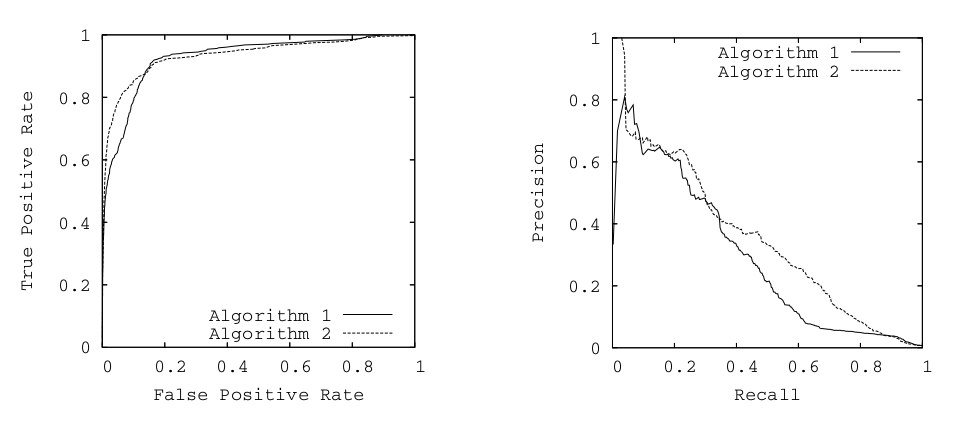
\includegraphics[width = 0.83\textwidth]{plots/AUCandPRAUC.png}
	\caption[Sample ROC and PR curves]{A sample receiver operating characteristic curve (left) and precision-recall curve (right). Each algorithm is evaluated on different thresholds and the points produced are used to obtain the curves. Image courtesy of~\cite{Davis2006}}
	\label{fig:AUCandPRAUC}
\end{figure}

For unbalanced data sets, ``using the classifiers produced by standard machine learning algorithms without adjusting the output threshold may well be a critical mistake''~\cite{Provost2000}. It is preferable to use metrics that consider all possible thresholds (AUC or PRAUC) or simpler metrics ($F_1$ score or G-mean) with a threshold obtained via a validation set. The metric used for model selection influences its characteristics and behaviour, hence, it should be chosen carefully: we favor the use of PRAUC over AUC as well as $F_1$ score over G-mean because they concentrate in the positive class (disease) that is more interesting and harder to predict. Furthermore, PRAUC has been shown to have better properties than AUC in unbalanced data sets~\cite{Davis2006}. % In general, results for all these metrics.
We introduce metrics tailored to image segmentation models in Sec.~\ref{sec:Segmentation}.
%F1 better represents a more balanced tradeoff  (an small change in precision is corresponded with a small change in recall) than AUC where an small change in specificity can be corresponded with a big change in sensitivity.

\begin{comment} Discussion of why G-mean over F1
(Not sure about this) As a rule of thumb, using G-mean will generate models that predict more positives given that the sensitivity will greatly improve and specificity will only slightly decrease. Using $F_1$ score, the model will predict less positives as that will improve precision but only slightly decrease sensitivity. 
5 here say PRAUc is better for unbalanced classes

Why G-means? Because it is more important to obtain a low error in specificity than in precision, i .e, would you prefer a 90% in specificity or a 90% in precision?. 90% in specificity means that 10% of actual negatives (10 persons) were told they have no cancer although they actually had cancer, meanwhile 10% of expected positives(a small number, maybe 1) was said he has cancer although he doesn{t. First is worse.

Using G-mean i will predict more positives, no matter what. My sensitivity is going to vastly improve and the specificity will only decrease a little, but the precision is gonna take a hit. Because if I predict less positives sensitivity is gonna go down, specificity is gonna go up (as I add more true negatives) but just a little and precision  would go up (but it wouldn't matter for g-mean).

Using F1 I'll probably predict less positives, sensitivity is going to go slightly down, and precision is going to go up, specificity doesn{t matter but it will decrease a little. Or I'll probably predcit as many poositives as needed. It focuses more on the positive class.

Other diagonal, the algorithm will learn negatives pretty well, so the one that predicts less positives(f1) probably isn{t learning much (it is predicting all negative).
\end{comment}

%We point out that this section introduces basic concepts in machine learning but leaves aside many practical details. Content and notation is based on materials from Stanford's Machine Learning course~\cite{Ng2014}.
